\ifx\wholebook\relax \else

\documentclass[UTF8]{article}

%
% loading packages
%

\RequirePackage{ifpdf}
\RequirePackage{ifxetex}

%
%
\ifpdf
  \RequirePackage[pdftex,%
       bookmarksnumbered,%
              colorlinks,%
          linkcolor=blue,%
              hyperindex,%
        plainpages=false,%
       pdfstartview=FitH]{hyperref}
\else\ifxetex
  \RequirePackage[bookmarksnumbered,%
               colorlinks,%
           linkcolor=blue,%
               hyperindex,%
         plainpages=false,%
        pdfstartview=FitH]{hyperref}
\else
  \RequirePackage[dvipdfm,%
        bookmarksnumbered,%
               colorlinks,%
           linkcolor=blue,%
               hyperindex,%
         plainpages=false,%
        pdfstartview=FitH]{hyperref}
\fi\fi
%\usepackage{hyperref}

% other packages
%--------------------------------------------------------------------------
\usepackage{graphicx, color}
\usepackage{wrapfig}
\usepackage{subfig}
\usepackage{multicol}
\usepackage{tikz}
\usetikzlibrary{matrix,positioning,shapes}
\usetikzlibrary{patterns}

\usepackage{amsmath, amsthm, amssymb} % for math
\usepackage{exercise} % for exercise
\usepackage{import} % for nested input

%
% for programming
%
\usepackage{verbatim}
\usepackage{fancyvrb}
\usepackage{listings}
%\usepackage{algorithmic} %old version; we can use algorithmicx instead
%\usepackage[plain]{algorithm} %remove rule (horizontal line on top/below the algorithm
\usepackage{algorithm} %to remove rules change to \usepackage[plain]{algorithm}
%\usepackage{algorithm2e}
\usepackage[noend]{algpseudocode} %for pseudo code, include algorithmicsx automatically
\usepackage{appendix}
\usepackage{makeidx} % for index support
\usepackage{titlesec}
\usepackage{epigraph}

\usepackage[cm-default]{fontspec}
\usepackage{xunicode}
%\usepackage{fontenc}
\usepackage{textcomp}
\usepackage{url}

% detect and select Chinese font
% ------------------------------
% fc-list :lang=zh    % list all Chinese fonts
% fc-list :mono       % list all mono fonts
% fc-cache            % refresh cache to load new installed fonts
\def\macmainfont{STSong}  % Under Mac OS X
\def\macmonofont{Monaco}
\def\winmainfont{SimSun} % Under Windows
\def\winmonofont{Consolas}
\def\linuxmainfont{WenQuanYi Micro Hei} % Under Linux
\def\linuxmainfont{Courier}

\suppressfontnotfounderror1 % Avoid setting exit code (error level) to break make process
\count255=\interactionmode
\batchmode

% main font
\let\mainft=\macmainfont
\font\thefont="\mainft"\space at 10pt
\ifx\thefont\nullfont
  \let\mainft=\winmainfont
  \font\thefont="\mainft"\space at 10pt
  \ifx\the\nullfont
    \let\mainft=\linuxmainfont
    \font\thefont="\mainft"\space at 10pt
    \ifx\the\nullfont
      \errorstopmode
      \errmessage{no suitable Chinese main font found}
    \fi
  \fi
\fi

% mono font
\let\monoft=\macmonofont
\font\thefont="\monoft"\space at 10pt
\ifx\thefont\nullfont
  \let\monoft=\winmonofont
  \font\thefont="\monoft"\space at 10pt
  \ifx\the\nullfont
    \let\monoft=\linuxmonofont
    \font\thefont="\monoft"\space at 10pt
    \ifx\the\nullfont
      \errorstopmode
      \errmessage{no suitable mono font found}
    \fi
  \fi
\fi

\interactionmode=\count255

\setmainfont[Mapping=tex-text]{\mainft}
\setmonofont[Scale=MatchLowercase]{\monoft}   % 英文等宽字体

\XeTeXlinebreaklocale "zh"  % to solve the line breaking issue
\XeTeXlinebreakskip = 0pt plus 1pt minus 0.1pt

\titleformat{\paragraph}
{\normalfont\normalsize\bfseries}{\theparagraph}{1em}{}
\titlespacing*{\paragraph}
{0pt}{3.25ex plus 1ex minus .2ex}{1.5ex plus .2ex}

\lstdefinelanguage{Smalltalk}{
  morekeywords={self,super,true,false,nil,thisContext}, % This is overkill
  morestring=[d]',
  morecomment=[s]{"}{"},
  alsoletter={\#:},
  escapechar={!},
  literate=
    {BANG}{!}1
    {UNDERSCORE}{\_}1
    {\\st}{Smalltalk}9 % convenience -- in case \st occurs in code
    % {'}{{\textquotesingle}}1 % replaced by upquote=true in \lstset
    {_}{{$\leftarrow$}}1
    {>>>}{{\sep}}1
    {^}{{$\uparrow$}}1
    {~}{{$\sim$}}1
    {-}{{\sf -\hspace{-0.13em}-}}1  % the goal is to make - the same width as +
    %{+}{\raisebox{0.08ex}{+}}1		% and to raise + off the baseline to match -
    {-->}{{\quad$\longrightarrow$\quad}}3
	, % Don't forget the comma at the end!
  tabsize=2
}[keywords,comments,strings]

% for literate Haskell code
\lstdefinestyle{Haskell}{
  flexiblecolumns=false,
  basewidth={0.5em,0.45em},
  morecomment=[l]--,
  literate={+}{{$+$}}1 {/}{{$/$}}1 {*}{{$*$}}1 {=}{{$=$}}1
           {>}{{$>$}}1 {<}{{$<$}}1 {\\}{{$\lambda$}}1
           {\\\\}{{\char`\\\char`\\}}1
           {->}{{$\rightarrow$}}2 {>=}{{$\geq$}}2 {<-}{{$\leftarrow$}}2
           {<=}{{$\leq$}}2 {=>}{{$\Rightarrow$}}2
           {\ .}{{$\circ$}}2 {\ .\ }{{$\circ$}}2
           {>>}{{>>}}2 {>>=}{{>>=}}2
           {|}{{$\mid$}}1
}

% "define" Scala
\lstdefinelanguage{Scala}{
  morekeywords={abstract,case,catch,class,def,%
    do,else,extends,false,final,finally,%
    for,if,implicit,import,match,mixin,%
    new,null,object,override,package,%
    private,protected,requires,return,sealed,%
    super,this,throw,trait,true,try,%
    type,val,var,while,with,yield},
  otherkeywords={=>,<-,<\%,<:,>:,\#,@},
  sensitive=true,
  morecomment=[l]{//},
  morecomment=[n]{/*}{*/},
  morestring=[b]",
  morestring=[b]',
  morestring=[b]"""
}

\lstloadlanguages{C, C++, Java, Lisp, Haskell, Python, Smalltalk, Scala}

\lstset{
  basicstyle=\small\ttfamily,
  commentstyle=\rmfamily,
  texcl=true,
  showstringspaces = false,
  upquote=true,
  flexiblecolumns=false
}

\newcommand\doubleplus{+\kern-1.3ex+\kern0.8ex}

% ======================================================================

\def\BibTeX{{\rm B\kern-.05em{\sc i\kern-.025em b}\kern-.08em
    T\kern-.1667em\lower.7ex\hbox{E}\kern-.125emX}}

%
% mathematics
%
\newcommand{\be}{\begin{equation}}
\newcommand{\ee}{\end{equation}}
\newcommand{\bmat}[1]{\left( \begin{array}{#1} }
\newcommand{\emat}{\end{array} \right) }
\newcommand{\VEC}[1]{\mbox{\boldmath $#1$}}

% numbered equation array
\newcommand{\bea}{\begin{eqnarray}}
\newcommand{\eea}{\end{eqnarray}}

% equation array not numbered
\newcommand{\bean}{\begin{eqnarray*}}
\newcommand{\eean}{\end{eqnarray*}}

\newtheorem{theorem}{定理}[section]
\newtheorem{lemma}[theorem]{引理}
\newtheorem{proposition}[theorem]{Proposition}
\newtheorem{corollary}[theorem]{Corollary}

% 中文书籍设置
% ====================================
\renewcommand\contentsname{目\ 录}
%\renewcommand\listfigurename{插图目录}
%\renewcommand\listtablename{表格目录}
\renewcommand\figurename{图}
\renewcommand\tablename{表}
\renewcommand\proofname{证明}
\renewcommand\ExerciseName{练习}
%\renewcommand{\algorithmcfname}{算法}

\ifx\wholebook\relax
\renewcommand\bibname{参\ 考\ 文\ 献}                    %book类型
%\newtheorem{Definition}[Theorem]{定义}
\newtheorem{Theorem}{定理}[chapter]
\newtheorem{example}{例题}[chapter]
\else
\renewcommand\refname{参\ 考\ 文\ 献}
\fi

%\setcounter{secnumdepth}{4}
\titleformat{\chapter}
  {\normalfont\bfseries\Large}
  {第\arabic{chapter}章}
  {12pt}{\Large}
%% \titleformat{\subsection}
%%   {\normalfont\bfseries\large}
%%   {\CJKnumber{\arabic{subsection}}、}
%%   {12pt}{\large}
%% \titleformat{\subsubsection}
%%   {\normalfont\bfseries\normalsize}
%%   {\arabic{subsubsection}.}
%%   {12pt}{\normalsize}

%\renewcommand{\baselinestretch}{1.5}                        %文章行间距为1.5倍。

\makeatletter
\newcommand{\verbatimfont}[1]{\renewcommand{\verbatim@font}{\ttfamily#1}}
\makeatother

\setcounter{tocdepth}{4}
\setcounter{secnumdepth}{4}

%\verbatimfont{\footnotesize}


\setcounter{page}{1}

\begin{document}

\title{递归}

\author{刘新宇
\thanks{{\bfseries 刘新宇} \newline
  Email: liuxinyu95@gmail.com \newline}
  }

\maketitle
\fi

\markboth{递归}{编程的数学原理}

\epigraph{\textbf{造物神}是\textbf{造}物主\textbf{物}色的\textbf{神}怪}{——[美]侯世达《哥德尔、埃舍尔、巴赫——集异壁之大成》}

\begin{wrapfigure}{R}{0.3\textwidth}
%\begin{figure}[htbp]
 \centering
 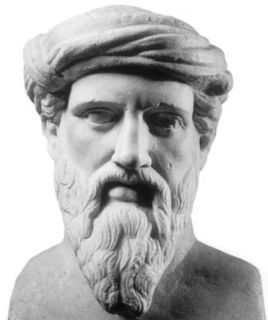
\includegraphics[scale=0.4]{img/Pythagoras.eps}
 \captionsetup{labelformat=empty}
 \caption{毕达哥拉斯(约前570——前490)}
 \label{fig:Pythagoras}
%\end{figure}
\end{wrapfigure}

人们通过深入了解数进而了解自然。在上一章中,我们介绍了自然数的皮亚诺公理。并且展示了一些和自然数有着相同结构的事物,包括计算机系统中的基本数据结构列表。自然数成为了我们进一步前进的基石。但是我们的大厦还不稳固。第一章中,我们不加证明地使用了递归的概念。例如阶乘的定义:

\[
\begin{array}{l}
fact(0) = 1 \\
fact(n + 1) = (n + 1) \cdot fact(n)
\end{array}
\]

以及$foldn$的实现:

\[
\begin{array}{l}
foldn(z, f, 0) = z \\
foldn(z, f, n') = f(foldn(z, f, n))
\end{array}
\label{eq:foldn}
\]

递归的原理是什么?为什么它是正确的?递归可以在更低的层次被表示么?这些都是我们在这一章要解决的问题。

\section{万物皆数}

从数出发研究世间万物的第一人要算是古希腊的数学家和哲学家毕达哥拉斯了。他的名字通过著名的勾股定理(在西方叫毕达哥拉斯定理)而家喻户晓。毕达哥拉斯出生于希腊的萨摩斯(Samos)岛,年轻时他曾去米利都(Miletus)向古希腊哲学的奠基人泰勒斯(Thales)学习。在泰勒斯的建议下,毕达哥拉斯前往东方学习数学。他在埃及学习了13年(一说为22年)。后来波斯帝国征服了埃及,他又随军向东到达了巴比伦,向巴比伦人学习数学和天文知识。或许后来他还到达了更远的印度。不论到了哪里,毕达哥拉斯都不断向有学问的人请教,丰富自己的见解。重要的是,他不仅刻苦学习,而且更善于思考。在经过兼收并蓄、汲取各家之长后,毕达哥拉斯形成并完善了自己的思想\cite{HanXueTao16}。

经历了漫长的在外游历后,这位年近半百的智者返回了故乡并开始讲学。公元前520年左右,为了摆脱当地的暴政,毕达哥拉斯移居到了意大利南部的克罗顿(Croton)发展,在那里他赢得了人们的信任与景仰。毕达哥拉斯的弟子中还有女性,他们把主要的精力都用来研究天文、几何、数论及音乐这四门学科。它们被称为四术(quadrivium),影响了欧洲教育两千多年\cite{StepanovRose15}。四术体现了毕达哥拉斯“万物皆数”的哲学思想。星体的运动与几何对应,而几何又以数为基础,数字还可以衍生出音乐。毕达哥拉斯是首个发现纯八度音(octave)在频率上有数学规律的人。他的弟子说他可以“听见天界的乐音”\footnote{关于毕达哥拉斯的逝世的说法不一。他领导的学派具有很高的声誉和政治影响,引起了敌对派的忌恨。后来受到民主运动的冲击,学派在克罗顿的活动场所遭到破坏。有人认为毕达哥拉斯被暴徒杀害,也有人说他逃到梅塔蓬图姆(Metapontum)并度过余生。}。

毕达哥拉斯学派深入研究了数与数、数与自然之间的关系。这开启了数学的重要分支——数论。他们对正整数进行了分类,定义了奇数偶数、素数和数等。他们发现某些数的所有真因子\footnote{小于数本身的因子}之和恰好等于这个数本身,毕达哥拉斯学派称这样的数为完全数,并成功地找到两个\footnote{一说为完美数。经过欧几里得与欧拉的进一步工作,揭示了偶完全数的特征以及完全数和梅森素数的关系。到2018年,人们借助计算机共发现了50个梅森素数和完全数。}。最小的完全数是6,因为6 = 1 + 2 + 3,下一个是28(等于1 + 2 + 4 + 7 + 14)。毕达哥拉斯学派还发现了一大类“形数”(figurate number)\footnote{毕达哥拉斯学派的门徒通过在地上摆小石子来研究数字,英文的计算calculus一词就是从希腊文“石子”衍生出的\cite{HanXueTao16}。当他们把石子按照某种几何方式排列成图形时,就得到了形数。}。

\begin{figure}[htbp]
%\begin{wrapfigure}{R}{0.4\textwidth}
\centering
\begin{tikzpicture}[scale=0.5]
\filldraw (0, 0) circle (0.2);
\draw (0, -1) node{1};
\filldraw (2, 0) circle (0.2)
          (3, 0) circle (0.2)   (3, 1) circle (0.2);
\draw (2.5, -1) node{3};
\filldraw (5, 0) circle (0.2)
          (6, 0) circle (0.2)   (6, 1) circle (0.2)
          (7, 0) circle (0.2)   (7, 1) circle (0.2)   (7, 2) circle (0.2);
\draw (6, -1) node{6};
\filldraw (9, 0) circle (0.2)
          (10, 0) circle (0.2)    (10, 1) circle (0.2)
          (11, 0) circle (0.2)    (11, 1) circle (0.2)    (11, 2) circle (0.2)
          (12, 0) circle (0.2)    (12, 1) circle (0.2)    (12, 2) circle (0.2)    (12, 3) circle (0.2);
\draw (10.5, -1) node{10};
\end{tikzpicture}
\caption{三角形数(triangular number)}
\label{fig:triangular-num}
%\end{wrapfigure}
\end{figure}

\begin{figure}[htbp]
%\begin{wrapfigure}{R}{0.4\textwidth}
\centering
\begin{tikzpicture}[scale=0.5]
\draw (0, 1) circle (0.2);
\filldraw (0, 0) circle (0.2);
\draw (0, -1) node{2};

\draw (2, 1) circle (0.2)   (2, 2) circle (0.2)
      (3, 2) circle (0.2);
\filldraw (2, 0) circle (0.2)
          (3, 0) circle (0.2)   (3, 1) circle (0.2);
\draw (2.5, -1) node{6};

\draw (5, 1) circle (0.2)   (5, 2) circle (0.2)   (5, 3) circle (0.2)
      (6, 2) circle (0.2)   (6, 3) circle (0.2)
      (7, 3) circle (0.2);
\filldraw (5, 0) circle (0.2)
          (6, 0) circle (0.2)   (6, 1) circle (0.2)
          (7, 0) circle (0.2)   (7, 1) circle (0.2)   (7, 2) circle (0.2);
\draw (6, -1) node{12};

\draw (9, 1) circle (0.2)   (9, 2) circle (0.2)   (9, 3) circle (0.2)   (9, 4) circle (0.2)
      (10, 2) circle (0.2)   (10, 3) circle (0.2)   (10, 4) circle (0.2)
      (11, 3) circle (0.2)   (11, 4) circle (0.2)
      (12, 4) circle (0.2);
\filldraw (9, 0) circle (0.2)
          (10, 0) circle (0.2)    (10, 1) circle (0.2)
          (11, 0) circle (0.2)    (11, 1) circle (0.2)    (11, 2) circle (0.2)
          (12, 0) circle (0.2)    (12, 1) circle (0.2)    (12, 2) circle (0.2)    (12, 3) circle (0.2);
\draw (10.5, -1) node{20};
\end{tikzpicture}
\caption{长方形数(oblong number)}
\label{fig:oblong-num}
%\end{wrapfigure}
\end{figure}

图\ref{fig:triangular-num}和图\ref{fig:oblong-num}分别是三角形数和长方形数。很容易看出,每个长方形数都是对应三角形数的二倍,而三角形数又是前$n$个正数之和,因此就得到了正整数累加的求和公式:

\[
1 + 2 + 3 + ... + n = \frac{1}{2}n(n+1)
\]

毕达哥拉斯学派还观察到,所有的奇数可以标示成折尺形(数学上称为“磬折形”),如图\ref{fig:gnomon-num},而前$n$个折尺形可以拼成一个正方形,如图\ref{fig:square-num}。这样他们就发现了前$n$个正奇数的求和公式:

\[
1 + 3 + 5 + ... + (2n - 1) = n^2
\]

\begin{figure}[htbp]
%\begin{wrapfigure}{R}{0.4\textwidth}
\centering
\begin{tikzpicture}[scale=0.5]
\filldraw (0, 0) circle (0.2);
\draw (0, -1) node{1};

\draw (2, 1) circle (0.2)
      (3, 0) circle (0.2)   (3, 1) circle (0.2);
\draw (2.5, -1) node{3};

\filldraw (5, 2) circle (0.2)   (6, 2) circle (0.2)   (7, 2) circle (0.2)
          (7, 0) circle (0.2)   (7, 1) circle (0.2);
\draw (6, -1) node{5};

\draw (9, 3) circle (0.2)   (10, 3) circle (0.2)   (11, 3) circle (0.2)   (12, 3) circle (0.2)
      (12, 0) circle (0.2)    (12, 1) circle (0.2)    (12, 2) circle (0.2);
\draw (10.5, -1) node{7};
\end{tikzpicture}
\caption{折尺形数(gnomon number)}
\label{fig:gnomon-num}
%\end{wrapfigure}
\end{figure}

\begin{figure}[htbp]
%\begin{wrapfigure}{R}{0.4\textwidth}
\centering
\begin{tikzpicture}[scale=0.5]
\filldraw (0, 0) circle (0.2);
\draw (0, -1) node{1};

\filldraw (2, 0) circle (0.2);
\draw (2, 1) circle (0.2)
      (3, 0) circle (0.2)   (3, 1) circle (0.2);
\draw (2.5, -1) node{4};

\filldraw (5, 0) circle (0.2);
\draw (5, 1) circle (0.2)
      (6, 0) circle (0.2)   (6, 1) circle (0.2);
\filldraw (5, 2) circle (0.2)   (6, 2) circle (0.2)   (7, 2) circle (0.2)
          (7, 0) circle (0.2)   (7, 1) circle (0.2);
\draw (6, -1) node{9};

\filldraw (9, 0) circle (0.2);
\draw (9, 1) circle (0.2)
      (10, 0) circle (0.2)   (10, 1) circle (0.2);
\filldraw (9, 2) circle (0.2)   (10, 2) circle (0.2)   (11, 2) circle (0.2)
          (11, 0) circle (0.2)   (11, 1) circle (0.2);
\draw (9, 3) circle (0.2)   (10, 3) circle (0.2)   (11, 3) circle (0.2)   (12, 3) circle (0.2)
      (12, 0) circle (0.2)    (12, 1) circle (0.2)    (12, 2) circle (0.2);
\draw (10.5, -1) node{16};
\end{tikzpicture}
\caption{正方形数(square number)与折尺形数的关系}
\label{fig:square-num}
%\end{wrapfigure}
\end{figure}

这正是我们在第一章提出的那个练习题的答案。就这样,毕达哥拉斯学派发现,很多事物和现象都可以从数的方面进行说明和解释。例如,具有同样张力的两根弦,当它们的长度为简单的整数比时,奏出的乐声就和谐悦耳。由此毕达哥拉斯发展出了最初的音乐理论。音乐与数这似乎毫无关联的两者间存在的这种意外联系,给毕达哥拉斯很大影响。他从中得到启发并大胆推测:所有的事物都可以用整数或整数的比来解释。毕达哥拉斯学派开始热衷与用数去解释更多的现象,他们相信宇宙的本质就在于“数的和谐”,并且提出“万物皆数”的论断。由此出发,毕达哥拉斯学派试图发展一套以数字为基础的理论,使得几何学可以建立在该理论之上。这种想法实际上就相当于要创建一套基于正整数的统一数学理论。

毕达哥拉斯学派最著名的发现当属勾股定理的证明。至今这一定理在西方仍被称为“毕达哥拉斯定理”。然而,我们将看到勾股定理是一把双刃剑,他的结果最终形成了一个递归的怪圈,使得“万物皆数”的理念出现了漏洞。为此,我们先要引出可公度概念和欧几里得算法。为了将几何纳入“万物皆数”的理论,毕达哥拉斯学派提出了一个概念来定义一条线段可以用另一条线段来度量。这个定义说,如果一条线段A可以通过有限的连续的另一条线段V来表示时,线段V可用于线段A的量度(measure)。这本质上是说,我们可以通过整数次拼接产生另一条线段。尽管度量两条不同的线段时,可以使用各自的量度,但是如果想用同一量度测量不同的线段,它必须是二者的公度(common measure)。即当且仅当线段V可以同时成为线段A和线段B的量度时,它才能成为二者的公度。毕达哥拉斯学派认为,任何情况下都可以找到公度,这样几何就可以建立在整数之上了。

%\begin{wrapfigure}{R}{0.4\textwidth}
\begin{figure}[htbp]
 \centering
 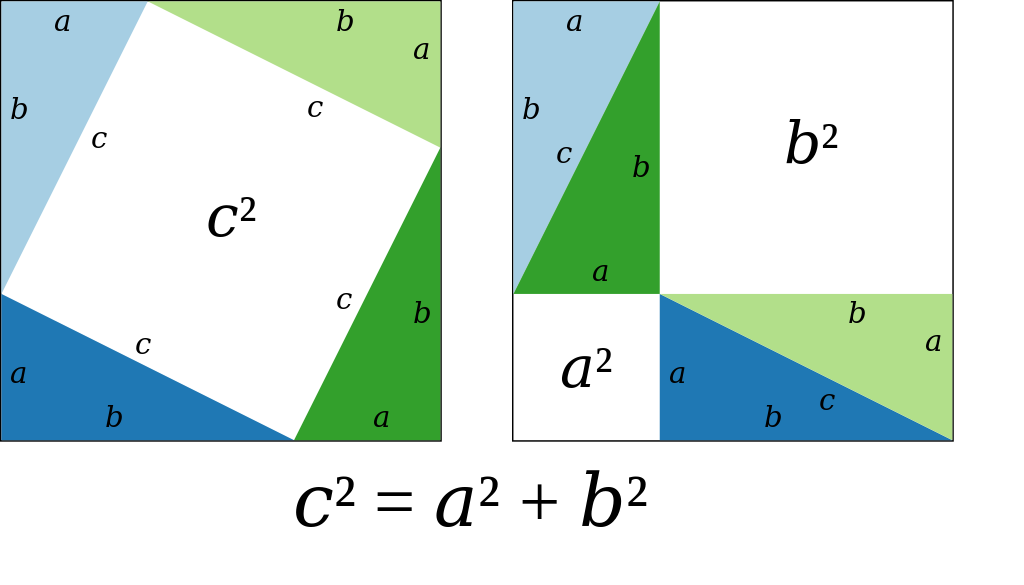
\includegraphics[scale=0.2]{img/Pythagoras-proof.eps}
 \caption{勾股定理的一种几何证明,两幅图中白色面积相等(来自《周髀算经》,约公元前200年)}
 \label{fig:Pythagoras-proof}
\end{figure}
%\end{wrapfigure}

\section{欧几里得算法}

由于公度可能有多个,为此需要引入最大公度(greatest common measure)的概念。如果线段V是线段A和线段B的公度,并且比其它公度都大,则称V是A和B的最大公度。已知两条线段,怎样才能求得最大公度呢?这就引出了历史上著名的递归算法——欧几里得算法(又称辗转相除法)。它用古希腊伟大的数学家欧几里得的名字命名\footnote{印度和中国分别独立发现了欧几里得算法。五世纪末,印度数学家阿耶波多(Aryabhata)用这一算法解不定方程(丢番图方程)。在《孙子算经》中,欧几里得算法可以作为中国剩余定理的特例。在1247年,南宋数学家秦九韶在《数书九章》中详细给出了欧几里得算法。}。在欧几里得的名著《几何原本》第十卷命题三中\cite{Elements},详细阐述了这一算法\footnote{在《几何原本》卷七的命题一中,有针对整数的欧几里得算法。但针对线段的情形实际上覆盖了整数。}。

\subsection{欧几里得和《几何原本》}

\begin{wrapfigure}{R}{0.4\textwidth}
%\begin{figure}[htbp]
 \centering
 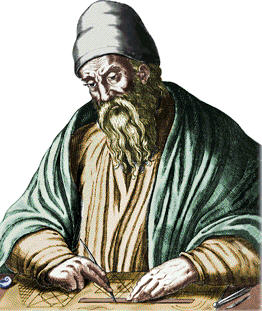
\includegraphics[scale=0.6]{img/Euclid.eps}
 \caption{欧几里得,约公元前300年前后}
 \label{fig:Peano}
%\end{figure}
\end{wrapfigure}

欧几里得(Euclid)是古希腊数学家,以其所著的《几何原本》闻名于世。对于他的生平,现在知道的很少。柏拉图学派晚期的导师普罗克洛斯(Proclus)在《几何学发展概要》中记述了这样的趣事:当时的埃及国王,亚历山大的托勒密一世有一次问欧几里得,学习几何学又没有什么捷径可走。欧几里得回答到:“在几何里,没有专为国王铺设的大道。”(There is no royal road to geometry)这句话成为千古传颂的学习箴言\footnote{也译为“几何无王者之道”}。斯托比亚斯(Stobaeus)记述另一则故事说。一个学生刚开始学习第一个命题,就问欧几里得学习几何后将得到什么。欧几里得说:“给他三个钱币,因为他想在学习中获取实利。”由此可知欧几里得主张学习必须循序渐进、刻苦钻研、不赞成投机取巧的作风,也反对狭隘实用观点\cite{Elements}。

欧几里得的《几何原本》是一部划时代的著作。其伟大的历史意义在于它是用公理建立起演绎体系的最早典范。过去所积累下来的数学知识是零碎的、片断的,可以比作木石砖瓦。只有借助于逻辑方法,把这些知识组织起来,加以分类比较,解释彼此间的内在联系,整理在一个严密的系统之中,才能建成巍峨的大厦。《几何原本》完成了这一艰巨的任务,它对整个数学的发展产生了深远的影响。

2000多年来,这部著作在几何教学中一直占据统治地位,在20世纪初依然用于数学课的基本教材。包括我国在内的许多国家仍将其作为中学的必修科目(现在中学的几何课本是按照法国数学家拉格朗日《几何原本》改写本思路编写的),并作为训练逻辑推理的最有力教育手段\cite{HanXueTao16}。

\subsection{欧几里得算法}

\begin{proposition}
《几何原本》,卷十,命题三:已知两个可公度的量,求它们的最大公度量。
\end{proposition}

欧几里得给出的方法,只需要使用递归和减法。因此,本质上求最大公度可以用尺规作图的方式给出。这一算法可以形式化如下。

\be
gcm(a, b) = \left \{
  \begin{array}
  {r@{\quad:\quad}l}
  a = b & a \\
  b < a & gcm(a - b, b) \\
  a < b & gcm(a, b - a)
  \end{array}
\right.
\label{eq:gcm-minus}
\ee

设两条线段$a$、$b$可公度,如果它们相等,则最大公度就是其中的任一条线段,此时算法返回$a$作为结果。如果线段$a$比$b$长,就用圆规不断从$a$中截去$b$(通过递归),然后求截短的线段$a'$和$b$的最大公度;否则如果线段$b$比$a$长,就反过来不断从$b$中截去$a$,然后求$a$和截短的线段$b'$的最大公度。图\ref{fig:line-seg-gcm}描述了这一算法作用于两条线段的计算步骤。我们也可将这一算法应用于整数42和30,并和处理线段的过程进行对比,如下表:

\begin{figure}[htbp]
\centering
\begin{tikzpicture}[scale=0.15]

\filldraw (0, 0) circle (0.5)   (30, 0) circle (0.5)   (42, 0) circle (0.5);
\draw (-8, 0) node{$a$} (0, 0) -- (42, 0);
\filldraw (0, -5) circle (0.5)   (30, -5) circle (0.5);
\draw (-8, -5) node{$b$} (0, -5) -- (30, -5);

\filldraw (0,  -15) circle (0.5)   (12, -15) circle (0.5);
\draw (-8, -15) node{$a'=a-b$} (0, -15) -- (12, -15);
\filldraw (0, -20) circle (0.5)   (12, -20) circle (0.5)   (24, -20) circle (0.5)   (30, -20) circle (0.5);
\draw (-8, -20) node{$b$} (0, -20) -- (30, -20);

\filldraw (0,  -30) circle (0.5)   (6, -30) circle (0.5)   (12, -30) circle (0.5);
\draw (-8, -30) node{$a'$} (0, -30) -- (12, -30);
\filldraw (0, -35) circle (0.5)   (6, -35) circle (0.5);
\draw (-8, -35) node{$b'=b-2a'$} (0, -35) -- (6, -35);

\filldraw (0,  -45) circle (0.5)   (6, -45) circle (0.5);
\draw (-8, -45) node{$a''=a'-b'$} (0, -45) -- (6, -45);
\filldraw (0, -50) circle (0.5)   (6, -50) circle (0.5);
\draw (-8, -50) node{$b'$} (0, -50) -- (6, -50);

\end{tikzpicture}
\caption{欧几里得算法的线段示意}
\label{fig:line-seg-gcm}
\end{figure}

\begin{tabular}{|l|l|l|}
\hline
$gcm(a, b)$ & $a$ & $b$ \\
\hline
$gcm(42, 30)$ & 42 & 30 \\
\hline
$gcm(12, 30)$ & 12 & 30 \\
\hline
$gcm(12, 18)$ & 12 & 18 \\
\hline
$gcm(12, 6)$ & 12 & 6 \\
\hline
$gcm(6, 6)$ & 6 & 6 \\
\hline
\end{tabular}

注意到将一个量$b$反复从另一个量$a$中减去,最后得到$a'$的过程恰好是带余数的除法的定义。即$a' = a - \lfloor a / b \rfloor$或记为$a'= a \bmod b$。因此我们可以用除法和求余运算代替原始欧几里得算法中的反复相减。此外,当一个量是另一个量的整倍数时,例如$b \leq a$且$b$可以整除$a$,我们立即知道最大公度为$b$。此时求余的结果$a \bmod b = 0$,为此我们可以定义$gcm(0, b) = gcm(b, 0) = b$。我们可以先比较$a$和$b$的大小,如果$a < b$就交换两个量。由于我们知道$a \bmod b$一定小于$b$, 所以我们下次递归时可以直接交换$gcm(b, a \bmod b)$。这样我们就得到了改进的欧几里得算法。

\be
gcm(a, b) = \left \{
  \begin{array}
  {r@{\quad:\quad}l}
  b = 0 & a\\
  \text{否则} & gcm(b, a \bmod b) \\
  \end{array}
\right.
\label{eq:gcm}
\ee

为什么这个算法可以求出最大公度呢?我们需要分两步来证明它的正确性。第一步我们要证明这一算法可以求出公度。设$b \leq a$,令整数$q_0$为商,$r_0$为余数,即$a = b q_0 + r_0$,如果$r_0$为零,算法就找到了公度,为此我们考虑$r_0$不为零的情况。此时可以进一步列出$b = r_0 q_1 + r_1$,类似地,只要余数不为零,我们可以一直列出这样的式子。

\[
\begin{array}{rcl}
a &=& b q_0 + r_0 \\
b &=& r_0 q_1 + r_1 \\
r_0 &=& r_1 q_2 + r_2 \\
r_1 &=& r_2 q_3 + r_3 \\
& & ...
\end{array}
\]

但只要$a$、$b$是可公度的,这些式子不会无限列下去。理由是每次都用圆规截取整数次,即商是整数。同时每次都保证余数小于除数。即$b > r_0 > r_1 > r_2 > ... > 0$,但是余数不可能小于零。由于起始值是有限的,故最终一定在有限步内得到$r_{n-2} = r_{n-1} q_n$。

接下来我们证明最后一步得到的$r_{n-1}$可以同时度量$a$和$b$。根据度量的定义,显然$r_{n-1}$可以度量$r_{n-2}$。然后考虑倒数第二式$r_{n-3} = r_{n-2} q_{n-1} + r_{n-1}$,由于$r_{n-1}$可以度量$r_{n-2}$,所以$r_{n-1}$也可以度量$r_{n-2} q_{n-1}$,自然它也可以度量$r_{n-2} q_{n-1} + r_{n-1}$,这个量恰好等于$r_{n-3}$。用同样的方法,我们可以向上逐一证明$r_{n-1}$可以度量每个式子左边,一直到$b$、$a$。这样我们就证明了欧几里得算法得到的答案$r_{n-1}$是$a$、$b$的公度。若最大公度为$g$,一定有$r_{n-1} \leq g$。

第二步我们要证明,任何$a$、$b$的公度$c$,一定也可以度量$r_{n-1}$。由于$c$是公度,因此$a$和$b$可以用它来表示,不妨记$a = mc$、$b = nc$,其中$m$、$n$都是整数。这样第一式$a = b q_0 + r_0$就可以写成$mc = ncq_0 + r_0$,我们得知$r_0 = (m - nq_0)c$,因此$c$也可以度量$r_0$。类似地,我们可以依次证明$c$可以度量$r_1$、$r_2$、……、$r_{n-1}$。这样我们就证明了任何公度都可以度量$r_{n-1}$,因此最大公度$g$也可以度量$r_{n-1}$,即$g \leq r_{n-1}$。

综合第一、第二步的结果,即$r_{n-1} \leq g$且$g \leq r_{n-1}$,我们得出最大公度$g = r_{n-1}$,也就是说欧几里得算法能够正确地给出最大公度。进一步,我们知道$g$是每一对量的最大公度,即:

\[
g = gcm(a, b) = gcm(b, r_1) = ... = gcm(r_{n-2}, r_{n-1}) = r_{n-1}
\]

\subsection{欧几里得算法的意义}

在“万物皆数”的哲学思想下,虽然欧几里得算法算法最初是为了寻找两个整数的最大公约数而产生的。但是经过欧几里得之手,算法却应用到了抽象的几何量上。从整数的最大公约数,到可公度量的最大公度,我们看到了几何量和数的分离\footnote{这也是我们使用gcm,而没有使用更常见的gcd(greatest common divisor)作为算法简写的原因。}。几何不仅没有建立在整数之上,反而独立发展,解决了整数之外的问题。以至于后来古希腊数学形成了这样的传统,任何关于数的结论,都需要给出几何的证明。这一传统直到十六世纪仍然影响着人们。意大利数学家卡尔丹(Gerolamo Cardano)\footnote{也译作卡尔达诺}在关于解三次、四次方程的著作《大术》(Ars Magna,1545年出版)中,仍然使用类似立方体填补法的几何论证\cite{HanXueTao2009}。

欧几里得算法是最著名的一个递归算法。德国数学家,解析数论创始人狄利克雷(Dirchlet)在他的著作《数论讲义》中评价到:“整个数论的结构都建立在同一个基础之上,这个基础就是最大公约数算法。”现代密码学的RSA加密算法\footnote{RSA算法是最早的一种公开密钥加密的非对称加密算法,RSA是1977年由罗纳德·李维斯特(Ron Rivest)、阿迪·萨莫尔(Adi Shamir)和伦纳德·阿德曼(Leonard Adleman)一起提出的。当时他们三人都在麻省理工学院工作。RSA就是他们三人姓氏开头字母拼在一起组成的。}直接使用了扩展欧几里得算法。

扩展欧几里得算法、倒水趣题。

几何量和数的分离。最大公约数算法的意义,递归原理问题的提出



无理数的发现和递归的关系。

\begin{Exercise}
\Question{我们给出的欧几里得算法是递归的,请消除递归,只使用循环实现欧几里得算法。}
\Question{大多数编程环境中的取模运算,要求除数、被除数都是整数。但是线段的长度不一定是整数,请实现一个针对线段的取摸运算。它的效率如何?}
\Question{我们在证明欧几里得算法正确性的过程中说:“每次都保证余数小于除数。即$b > r_0 > r_1 > r_2 > ... > 0$,但是余数不可能小于零。由于起始值是有限的,故最终算法一定中止。”为什么不会出现,$r_{n}$无限接近于零但不等于零的情况?算法一定会中止么?$a$和$b$是可公度的这一前提保证了什么?}
\end{Exercise}

\section{$\lambda$演算}

lambda的由来,三大变换:Alpha, Beta, Eta变换,变换与归约。


\begin{Exercise}
\begin{enumerate}
\item 一些lambda演算的练习
\end{enumerate}
\end{Exercise}

\section{递归的定义}

Y组合子和递归的定义
%% \begin{wrapfigure}{R}{0.4\textwidth}
%% %\begin{figure}[htbp]
%%  \centering
%%  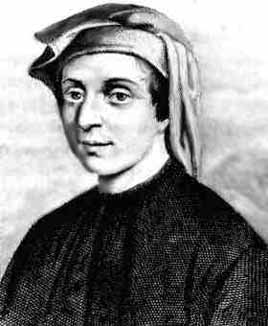
\includegraphics[scale=0.4]{img/Fibonacci.eps}
%%  \caption{比萨的列奥纳多,又称斐波那契(Leonardo Pisano, Fibonacci),1175年-1250年}
%%  \label{fig:Fibonacci}
%% %\end{figure}
%% \end{wrapfigure}


%\begin{wrapfigure}{L}{0.3\textwidth}
%% \begin{figure}[htbp]
%%  \centering
%%  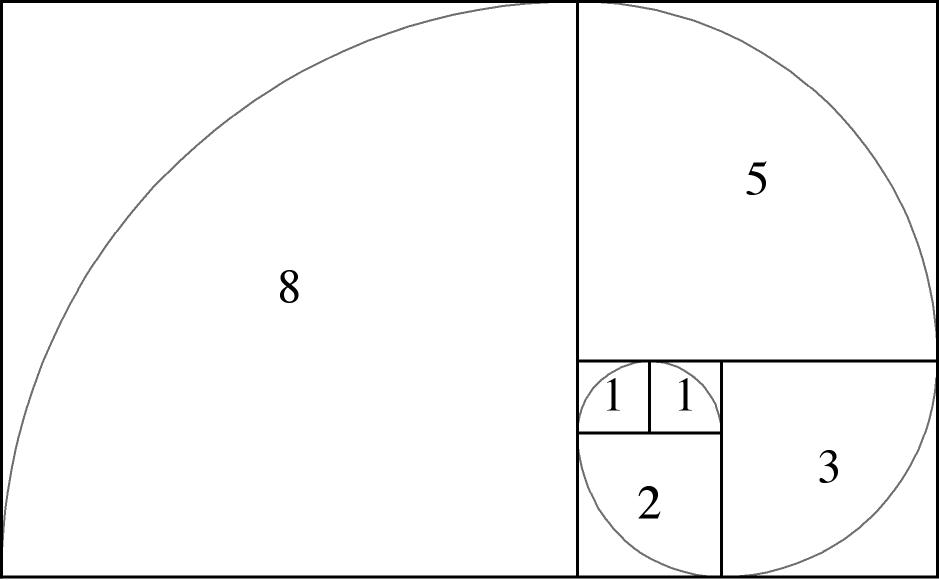
\includegraphics[scale=0.5]{img/fibonacci_spiral.eps}
%%  \caption{这些正方形的边长组成了斐波那契序列。}
%%  \label{fig:fibonacci_spiral}
%% \end{figure}
%\end{wrapfigure}

%\begin{wrapfigure}{R}{0.3\textwidth}
%% \begin{figure}[htbp]
%%  \centering
%%  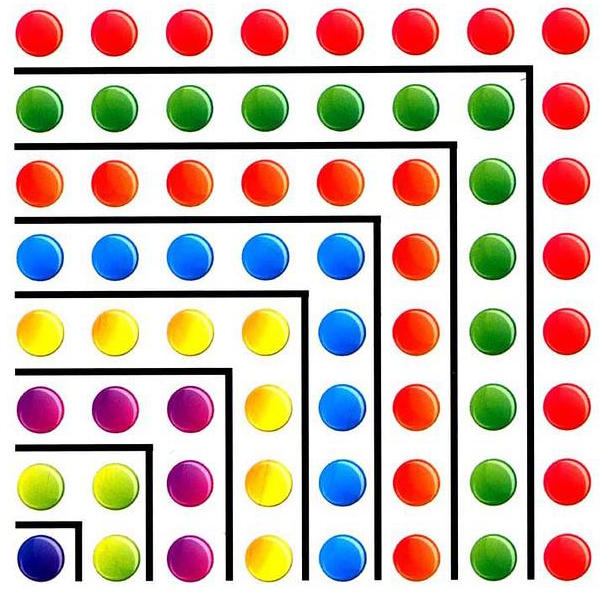
\includegraphics[scale=0.2]{img/PWW.eps}
%%  \caption{《无需语言的证明》封面局部}
%%  \label{fig:PWW}
%% \end{figure}
%\end{wrapfigure}

\section{$\lambda$的意义}

CONS/HEAD/TAIL的lambda表示。

二叉树、多叉树的递归结构与FOLD

\section{递归的结构与形式}

%\begin{wrapfigure}{R}{0.3\textwidth}
%% \begin{figure}[htbp]
%%  \centering
%%  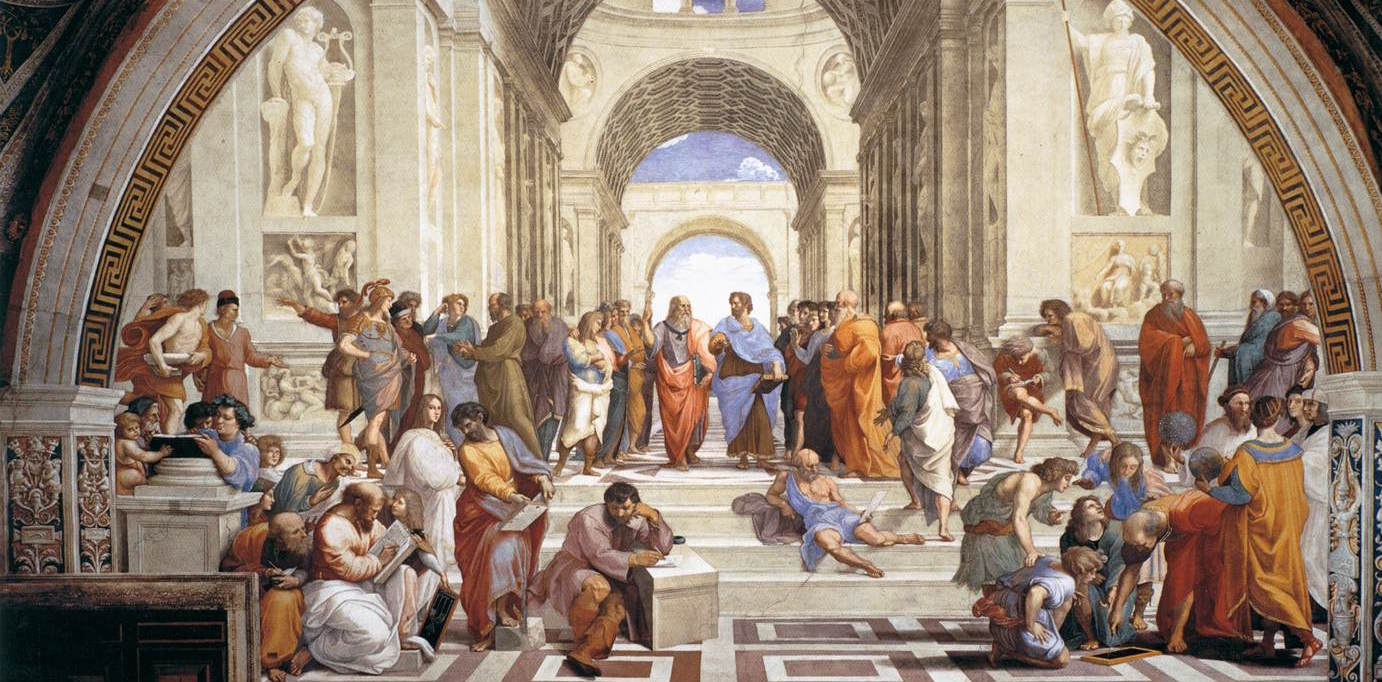
\includegraphics[scale=1.0]{img/the-school-of-athens.eps}
%%  \caption{拉斐尔《雅典学院》局部}
%%  \label{fig:the-school-of-athens}
%% \end{figure}
%\end{wrapfigure}

递归的形式之美——分形与艺术

递归的结构之美——文艺和音乐作品

\ifx\wholebook\relax \else
\begin{thebibliography}{99}

\bibitem{HanXueTao16}
韩雪涛 ``数学悖论与三次数学危机''. 人民邮电出版社. 2016, ISBN: 9787115430434

\bibitem{StepanovRose15}
[美] 亚历山大 A$cdot$斯捷潘诺夫,丹尼尔 E$\cdot$罗斯著,爱飞翔译. ``数学与泛型编程:高效编程的奥秘''. 机械工业出版社. 2017, ISBN: 9787111576587

\bibitem{Elements}
[古希腊] 欧几里得 著,兰纪正 朱恩宽 译,梁宗巨 张毓新 徐伯谦 校订 ``几何原本''. 译林出版社. 2014, ISBN: 9787544750066

\bibitem{Elements}
韩雪涛 ``好的数学——“下金蛋”的数学问题''. 湖南科学技术出版社. 2009, ISBN: 9787535756725

\end{thebibliography}

\expandafter\enddocument
%\end{document}

\fi
